\documentclass[pdf, intlimits, 9pt, unicode]{beamer}

\input{../config.tex}
\input{../header.tex}
\renewcommand{\docname}{Введение в машинное обучение}


\title[\disciplineshortname]{\docname}

\begin{document}

\maketitle

\begin{frame}<handout:0>{Содержание}\tableofcontents[pausesections]\end{frame}

\section{Пространство признаков}





\begin{frame}{Пространство признаков}
Мы видели что обучение {\color{red}(эмпирическое обобщение)} опирается на разные структуры данных.\pause

Структура системы машинного обучения определяет качество ответа на задачу анализа, но количественный ответ зависит от параметров модели, и чем их больше, тем...\pause

Мотивация снижения размерности задачи:

\begin{itemize}
\item Визуализация -- представить в голове 5-мерные данные довольно трудно\pause
\item Много признаков -- дольше обучать\pause
\item Качество обучения -- чтобы параметры были стабильными, данные должны быть из большой несмещённой выборки\pause
\item Небольшие модели экономнее при эксплуатации
\end{itemize}

\end{frame}





\begin{frame}{Локализованные параметры}\begin{center}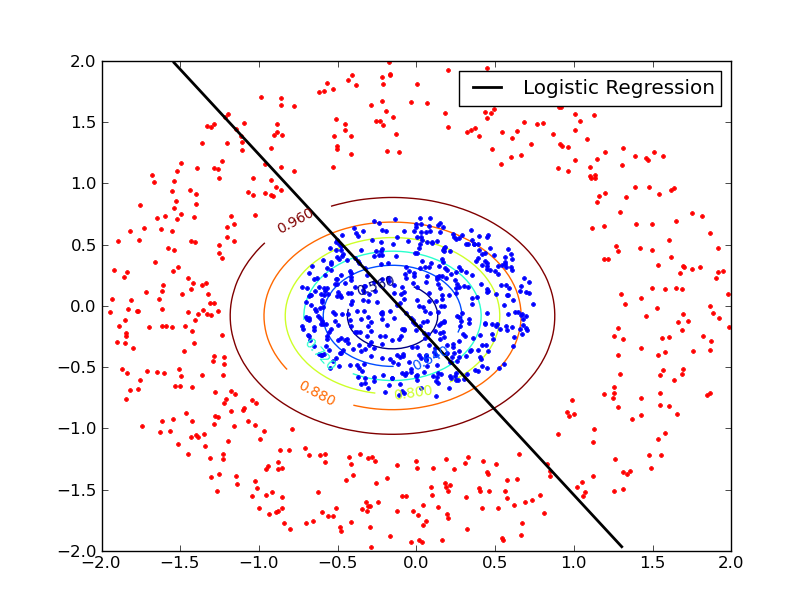
\includegraphics[height=.95\textheight]{xtC6P.png}\end{center}\end{frame}

\begin{frame}{Локализованные параметры}\begin{center}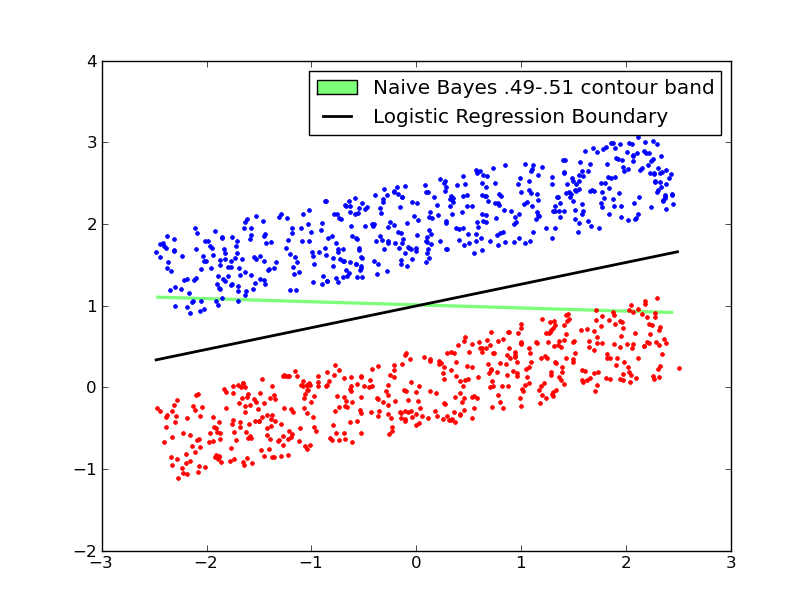
\includegraphics[height=.95\textheight]{3rkIp.png}\end{center}\end{frame}

\begin{frame}{Локализованные параметры}\begin{center}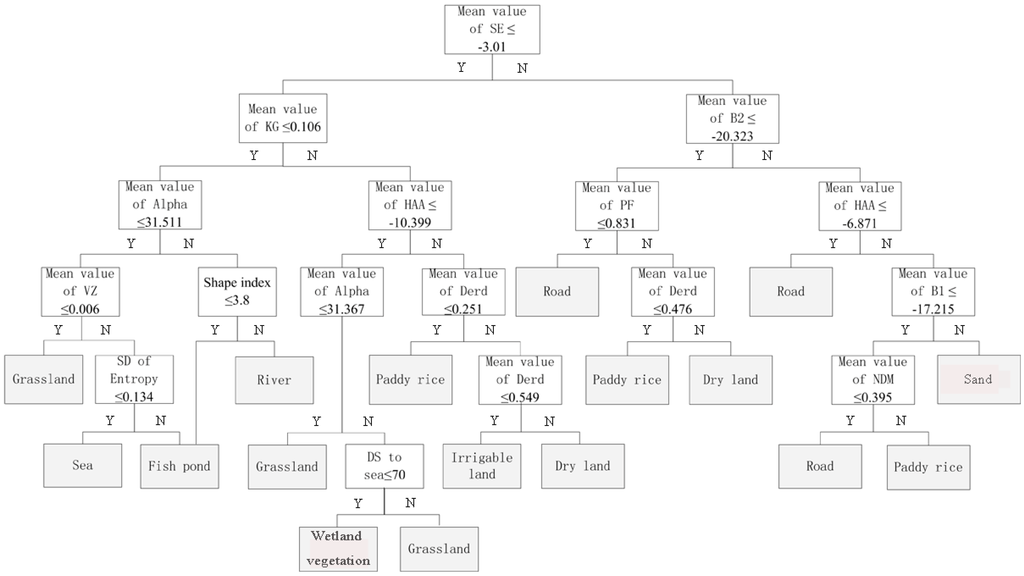
\includegraphics[width=.95\textwidth]{remotesensing-06-12575-g005-1024.png}\end{center}\end{frame}

\begin{frame}{Локализованные параметры}\begin{center}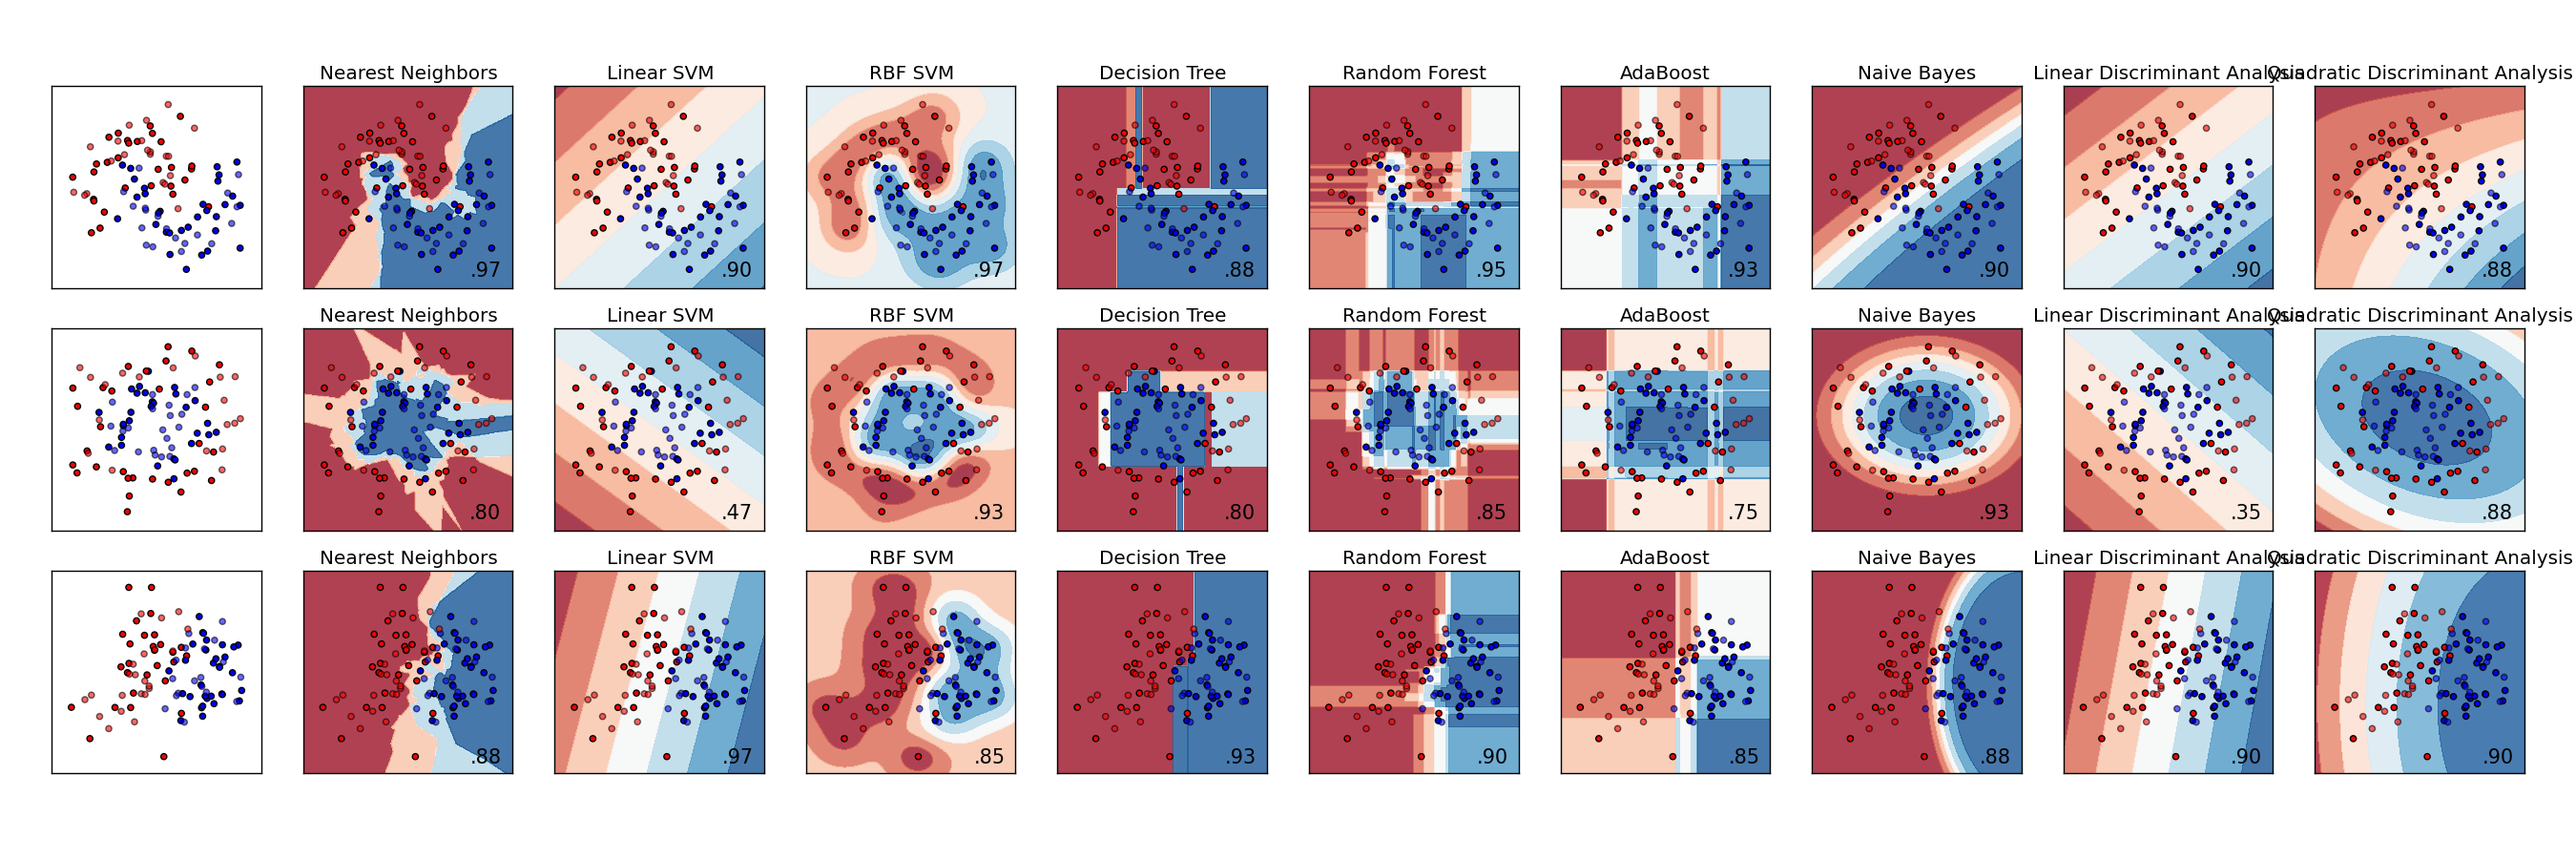
\includegraphics[width=.95\textwidth]{plotclassifiercomparison001.png}\end{center}\end{frame}





\begin{frame}{Признаки и обучение с учителем}\begin{center}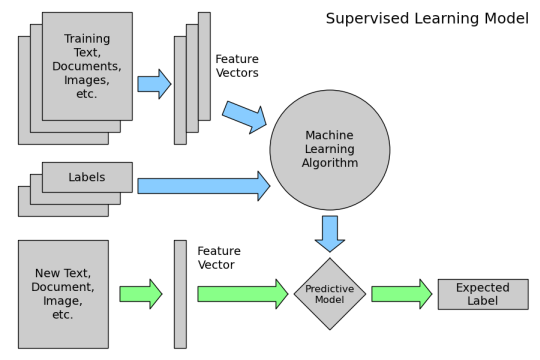
\includegraphics[width=.8\textwidth]{01_supervised_learning.png}\end{center}\end{frame}





% https://ru.wikipedia.org/wiki/%D0%97%D0%B0%D0%B4%D0%B0%D1%87%D0%B0_%D0%BA%D0%BB%D0%B0%D1%81%D1%81%D0%B8%D1%84%D0%B8%D0%BA%D0%B0%D1%86%D0%B8%D0%B8

\begin{frame}
Каждый объект описывается набором своих характеристик, называемых {\color{red}признаками}. Признаки могут быть числовыми или нет.\pause

Признаком называется отображение $f : X \to D_f$\pause

где $D_f$ -- множество допустимых значений признака.\pause

Если заданы признаки $f_1,\dots,f_n$, то вектор ${\mathbf x} = (f_1(x),\dots,f_n(x))$ называется признаковым описанием объекта $x \in X$.\pause

Признаковые описания допустимо отождествлять с самими объектами. При этом множество $X = D_{f_1}\times\dots\times D_{f_n}$ называют признаковым пространством.
\end{frame}






\begin{frame}
В зависимости от характера множества $D_f$ признаки делятся на следующие типы:
\bigskip

\begin{itemize}
\item {\color{red}бинарный} признак: $D_f=\{0,1\}$\pause
\item {\color{red}номинальный} признак: $D_f$ -- конечное множество\pause
\item {\color{red}порядковый} признак: $D_f$ -- конечное упорядоченное множество\pause
\item {\color{red}количественный} признак: $D_f$ -- множество действительных чисел
\end{itemize}

\end{frame}






\begin{frame}
Кроме этого, ситуация с признаками бывает разной:

\begin{itemize}
\item признаки привязаны к точкам данных (распознавание чисел)\pause
\item признаки отражают связи между данными (синтаксический разбор предложения)\pause
\item отсутствие признаков -- lazy learning\pause
\end{itemize}

Признаковое описание -- наиболее распространённый случай входных данных.\pause

В реальности информация не разделена по признакам, их нужно синтезировать.
\end{frame}





\begin{frame}
Синтаксический разбор -- построение \emph{проективного дерева минимального веса}, где веса подбираются на основе большой модели разобранного вручную текста (см. \emph{Корпус русского языка}).

\begin{center}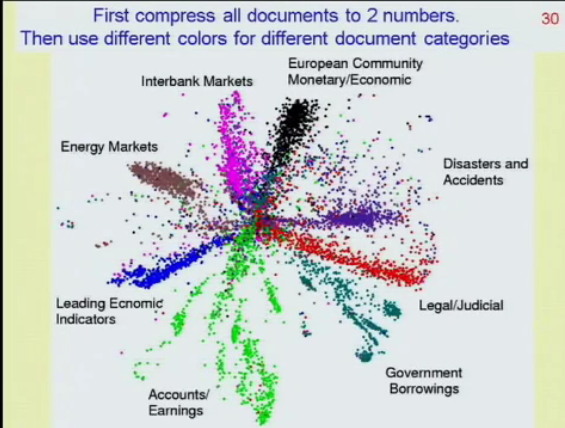
\includegraphics[width=\textwidth]{s1.png}\end{center}
\end{frame}




%\begin{frame}
%Обычно синтаксические деревья -- \emph{проективные}. Исключение -- поэзия и разговорная речь.
%
%\begin{center}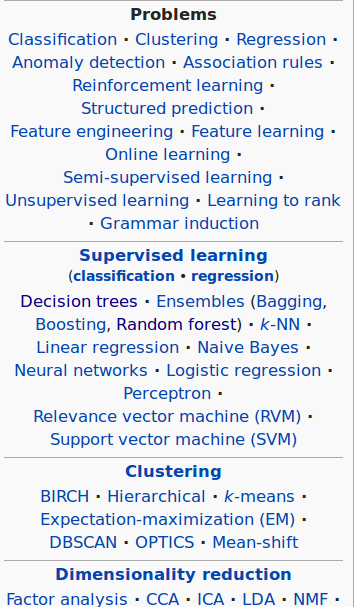
\includegraphics[width=.8\textwidth]{s2.png}\end{center}
%\end{frame}





\begin{frame}{Проклятие размерности}

\begin{center}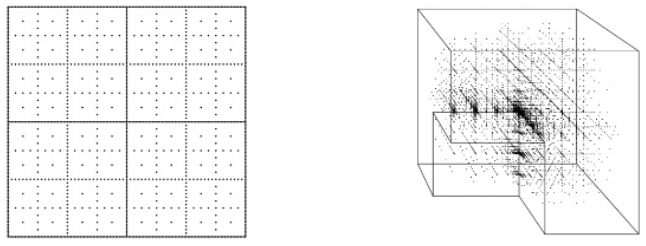
\includegraphics[width=.8\textwidth]{p000.png}\end{center}

\begin{itemize}
\item Сложность вычислений возрастает экспоненциально\pause
\item Требуется хранить огромное количество данных\pause
\item Большое число признаков являются шумными\pause
\item В линейных классификаторах увеличение числа признаков приводит к мультиколлинеарности и переобучению. Для метрических классификаторов (в пространствах с lp нормой) согласно закону больших чисел расстояния становятся неинформативны
\end{itemize}

\end{frame}










%http://www.youtube.com/watch?v=KY0A-f9e7N4
%http://habrahabr.ru/company/mailru/blog/254897/

\section{Методы подбора признаков}
\subsection{PCA}



%\begin{frame}\begin{center}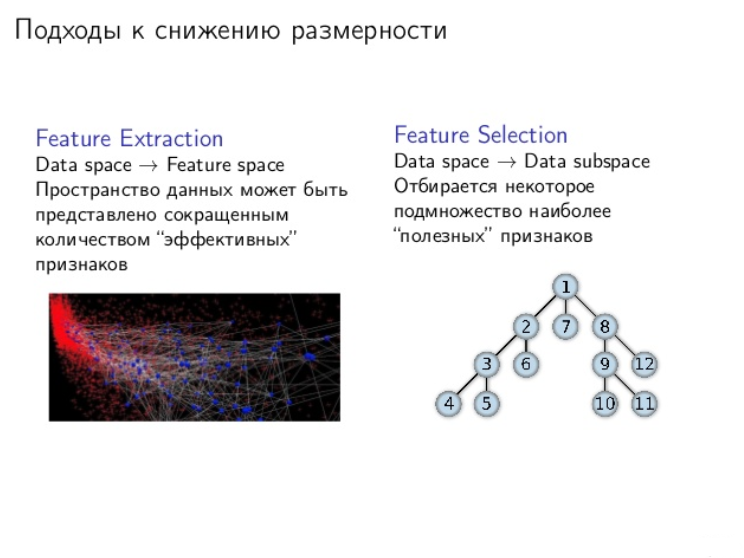
\includegraphics[width=\textwidth]{v01.png}\end{center}\end{frame}
\begin{frame}{Два подхода к снижению размерности}

\begin{columns}[t] %,onlytextwidth
\column{.5\textwidth}
\begin{block}{Feature extraction}
Data space $\rightarrow$ Feature space\\
Пространство данных может быть представлено сокращённым количеством <<эффективных>> признаков
\end{block}
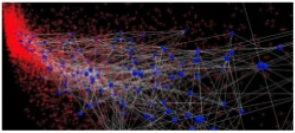
\includegraphics[width=\textwidth]{p010.png}\pause

\column{.5\textwidth}
\begin{block}{Feature Selection}
Data space $\rightarrow$ Data subspace\\
Отбирается некоторое подмножество наиболее <<полезных>> признаков
\end{block}
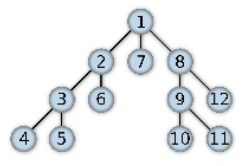
\includegraphics[width=\textwidth]{p011.png}
\end{columns}
\end{frame}





%\begin{frame}\begin{center}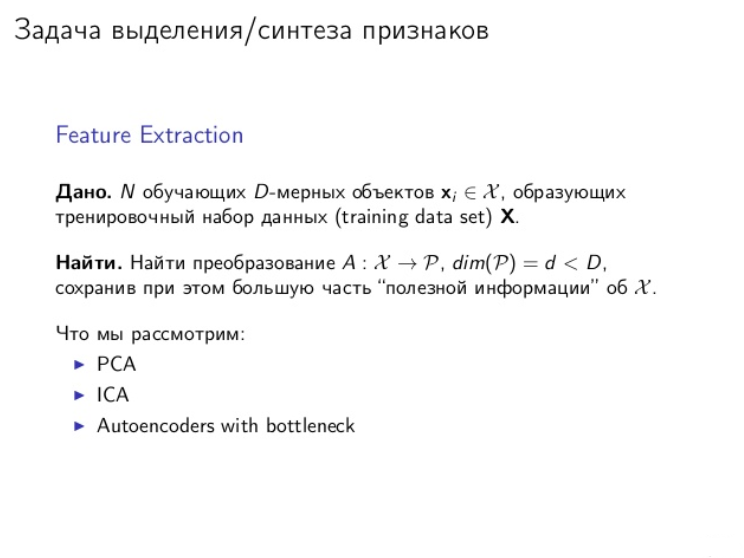
\includegraphics[width=\textwidth]{v02.png}\end{center}\end{frame}
\begin{frame}{Задача выделения/синтеза признаков}{Feature Extraction}

\textbf{Дано.} $N$ обучающих $D$-мерных объектов $x_i \in \mathscr{X}$, образующих тренировочный набор данных (training data set) $\mathbf{X}$.\pause

\textbf{Найти.} Найти преобразование $A : \mathscr{X} \to P$, $dim(P) = d < D$, сохранив при этом наибольшую часть <<полезной информации>> об $\mathscr{X}$.\pause

Что мы рассмотрим:

\begin{itemize}
\item PCA -- principal component analysis\pause
\item ICA -- independent component analysis\pause
\item Методы основанные на автоэнкодерах (autoencoders with bottlenecks)
\end{itemize}

\end{frame}





%\begin{frame}\begin{center}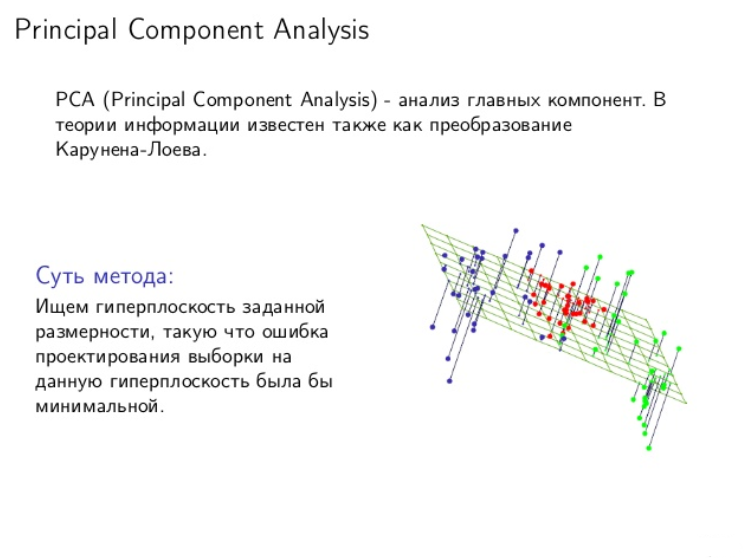
\includegraphics[width=\textwidth]{v03.png}\end{center}\end{frame}
\begin{frame}{Principal Component Analysis}

PCA (Principal Component Analysis) -- анализ главных компонент выборки. В теории информации также известен как \href{http://ru.wikipedia.org/wiki/Теорема_Карунена_—_Лоэва}{<<преобразование Карунена-Лоева>>}.\pause
\bigskip

\begin{columns}[c,onlytextwidth]
\column{.5\textwidth}
\begin{block}{Суть метода}
Находим гиперплоскость заданной размерности, такую что ошибка проектирования выборки на данную гиперплоскость будет минимальной.
\end{block}

\column{.5\textwidth}
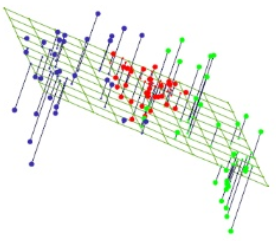
\includegraphics[width=\textwidth]{p020.png}
\end{columns}
\end{frame}




%\begin{frame}\begin{center}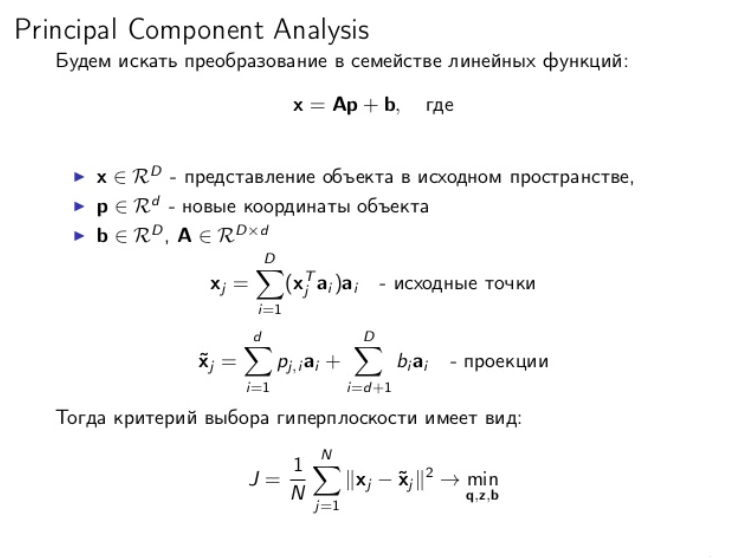
\includegraphics[width=\textwidth]{v04.png}\end{center}\end{frame}
\begin{frame}
Будем искать преобразование в семействе линейных функций:\pause

$$x = A p + b \text{, где}$$

\begin{itemize}
\item $x \in \mathscr{R}^D$ -- представление объекта в исходном пространстве\pause
\item $p \in \mathscr{R}^d$ -- новые координаты объекта\pause
\item $b \in \mathscr{R}^D$, $A \in \mathscr{R}^{D \times d}$ \pause
\end{itemize}

Исходные точки: $x_j = \sum_{i=1}^{D}{(x_j^T a_i)a_i}$\pause

Проекции: ${\tilde x}_j = \sum_{i=1}^{d}{p_{j,i} a_i} + \sum_{i=d+1}^{D}{b_i a_i}$\pause

Критерий выбора гиперплоскости:

$$J = \frac{1}{N} \sum_{j=1}^{N}{\| x_j - {\tilde x}_j\|^2 } \to \operatorname*{min}_{q,z,b}$$

\end{frame}




%\begin{frame}\begin{center}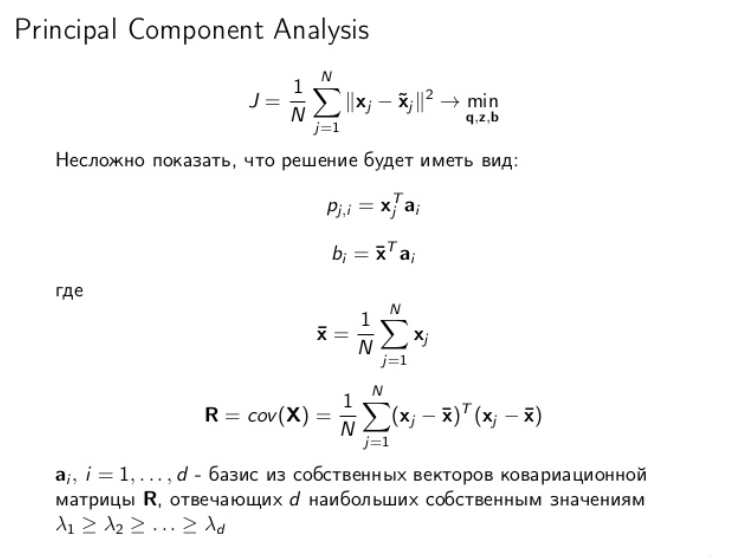
\includegraphics[width=\textwidth]{v05.png}\end{center}\end{frame}
\begin{frame}
Решение будет иметь вид:

$$p_{i,j} = x_j^T a_i$$

$$b_i = \bar{x}^T a_i$$

где

$$\bar{x} = \frac{1}{N} \sum_{j=1}^{N}{x_j}$$
\end{frame}





\begin{frame}
$$\mathbf{R} = cov(\mathbf{X}) = \frac{1}{N} \sum_{j=1}^{N}{(x_j - \bar x)^T (x_j - \bar x)}$$

$a_i, i = 1 \dots d$ -- базис из собственных векторов ковариационной матрицы $\mathbf{R}$, отвечающих $d$ наибольших собственным значениям $\lambda_1 \geq \lambda_1 \dots \geq \lambda_d$

\end{frame}






%\begin{frame}\begin{center}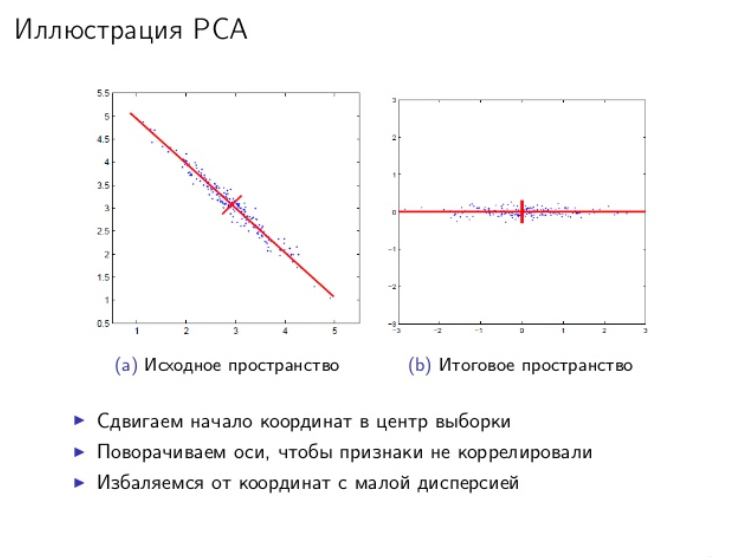
\includegraphics[width=\textwidth]{v06.png}\end{center}\end{frame}
\begin{frame}{Иллюстрация PCA}

\begin{center}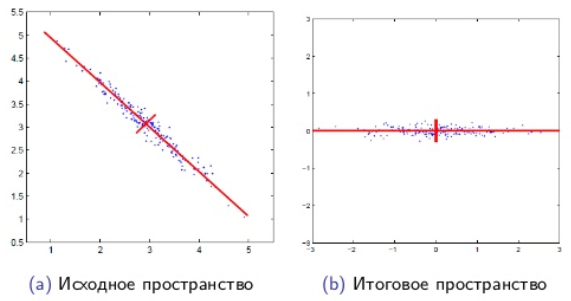
\includegraphics[width=.8\textwidth]{p060.png}\end{center}

\begin{itemize}
\item Сдвигаем начало координат в центр выборки\pause
\item Поворачиваем оси так, чтобы признаки не коррелировали\pause
\item Избавляемся от координат с малой дисперсией
\end{itemize}

\end{frame}




%\begin{frame}\begin{center}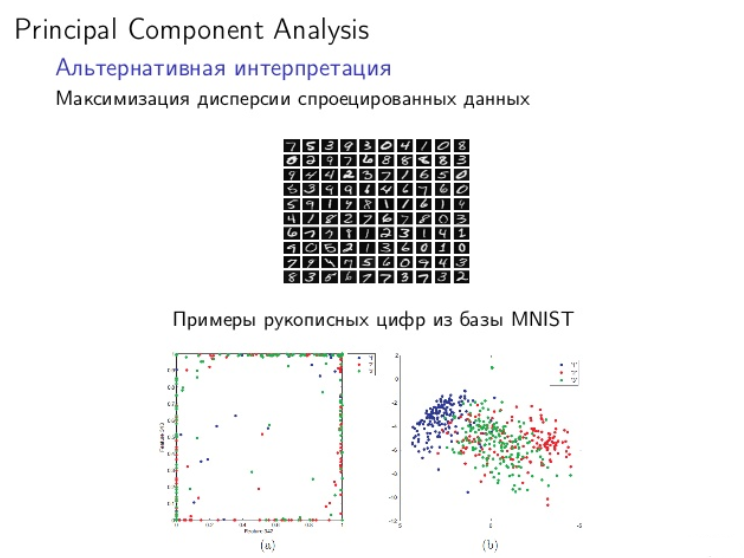
\includegraphics[width=\textwidth]{v07.png}\end{center}\end{frame}
\begin{frame}{Иными словами...}

PCA -- максимизация дисперсии проекции данных

\begin{center}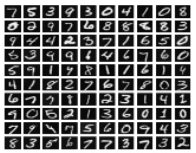
\includegraphics[width=.3\textwidth]{p070.png}\end{center}

Пример распознавания рукописных данных из \href{http://yann.lecun.com/exdb/mnist/}{БД MNIST}

\begin{center}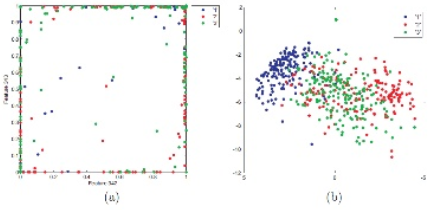
\includegraphics[width=.5\textwidth]{p071.png}\end{center}
\end{frame}





%\begin{frame}\begin{center}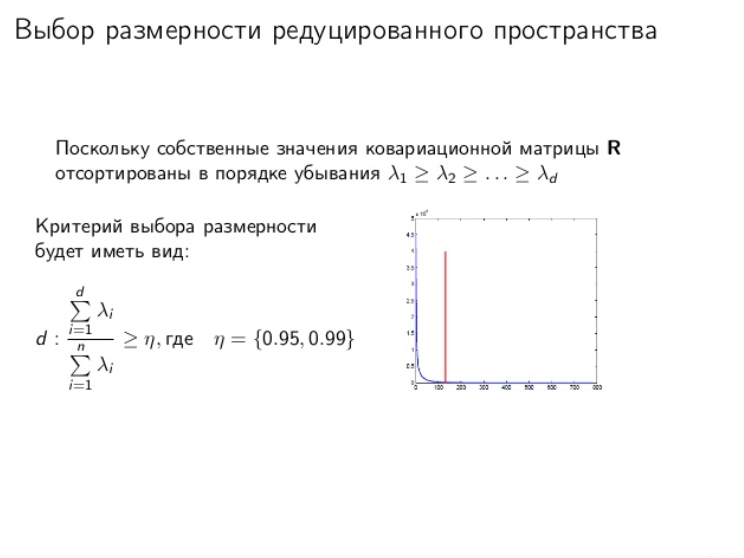
\includegraphics[width=\textwidth]{v08.png}\end{center}\end{frame}
\begin{frame}{Выбор размерности редуцированного пространства}
Поскольку собственные значения ковариационной матрицы $\mathbf{R}$ отсортированы в порядке убывания ($\lambda_1 \geq \lambda_1 \dots \geq \lambda_d$)\pause
\bigskip 
\begin{columns}[c,onlytextwidth]
\column{.5\textwidth}
критерий выбора размерности будет иметь вид:

$$d:\frac{\sum_{i=1}^{d}{\lambda_i}}{\sum_{i=1}^{n}{\lambda_i}} \leq \eta$$

где $\eta \in \{0.95 \dots 0.99\}$

\column{.5\textwidth}
\begin{center}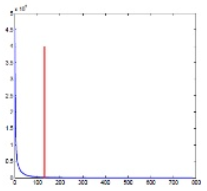
\includegraphics[width=.7\textwidth]{p080.png}\end{center}
\end{columns}
\end{frame}







%\begin{frame}\begin{center}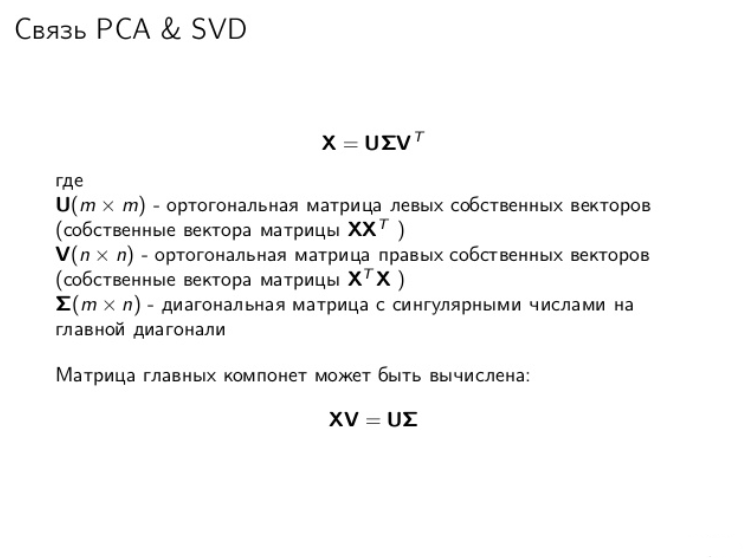
\includegraphics[width=\textwidth]{v09.png}\end{center}\end{frame}
\begin{frame}{Связь PCA и ICA}

$$X = U \Sigma V^T$$

где

\begin{itemize}
\item $U(m \times m)$ -- ортогональная матрица левых собственных векторов (собственные векторы матрицы $X X^T$)\pause
\item $V(n \times n)$ -- ортогональная матрица правых собственных векторов (собственные векторы матрицы $X^T X$)\pause
\item $\Sigma (m \times n)$ -- диагональная матрица с сингулярными числами на главной диагонали
\end{itemize}\pause

Матрица главных компонент может быть вычислена:

$$XV = U \Sigma$$

\end{frame}



\begin{frame}{Применение PCA}\begin{center}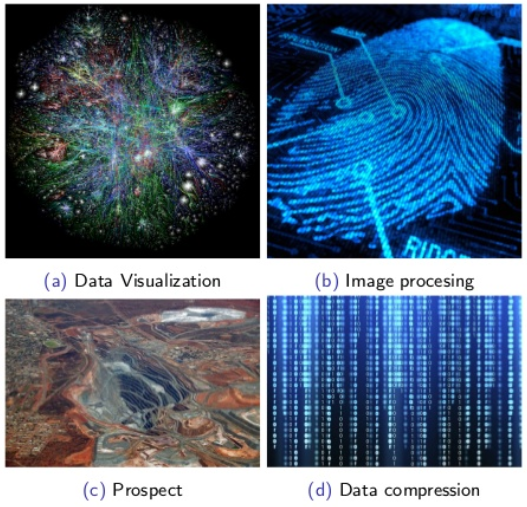
\includegraphics[height=\textheight]{PCA_Use.png}\end{center}\end{frame}



\begin{frame}{Достоинства и недостатки PCA}

\begin{itemize}
\item[$+$] Простой алгоритм
\item[$+$] Можно адаптировать для любого нелинейного случая, совершив преобразование ядра (см. Kernel trick)\pause
\item[$-$] Вычислять собственные веторы ковариационной матрицы в случае больших данных -- проблематично\pause
\item[$-$] Координаты объектов в новом пространстве неоднозначно определены
\end{itemize}\pause

\end{frame}




\subsection{ICA}

\begin{frame}<handout:0>{Задача слепого разделения сигналов}
\begin{center}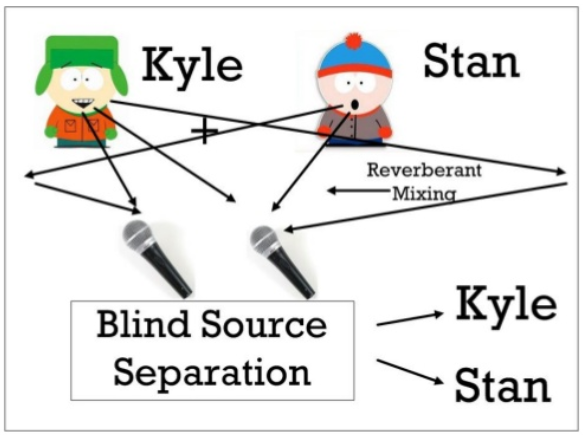
\includegraphics[width=\textwidth]{KyleStan.png}\end{center}
\end{frame}

%\begin{frame}\begin{center}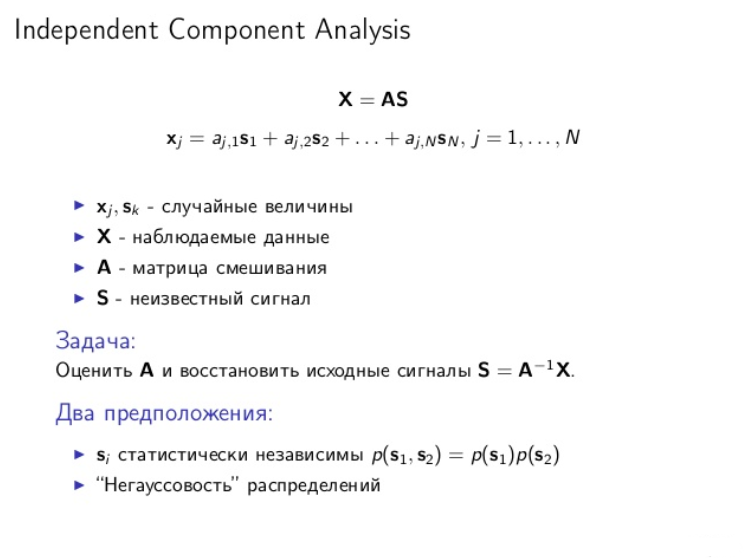
\includegraphics[width=\textwidth]{v13.png}\end{center}\end{frame}
\begin{frame}{ICA -- Анализ независимых компонентов}

$$X = A \cdot S$$

$$x_j = a_{j,1} s_1 + a_{j,2} s_2 + \dots + a_{j,N} s_N, j = 1, \dots, N$$

\begin{itemize}
\item $x_j$, $s_k$ -- случайные величины
\item $X$ -- наблюдаемые данные
\item $A$ -- матрица смешивания
\item {\color{red}$S$ -- неизвестный сигнал}
\end{itemize}\pause

\textbf{Задача:} Оценить $А$ и {\color{red}восстановить исходные сигналы} $S = A^{-1}X$\pause

\textbf{Два предположения:}

\begin{itemize}
\item $s_j$ -- статистически независимы $p(s_1,s_2) = p(s_1)p(s_2)$
\item не-гауссово распределение
\end{itemize}

\end{frame}




%\begin{frame}\begin{center}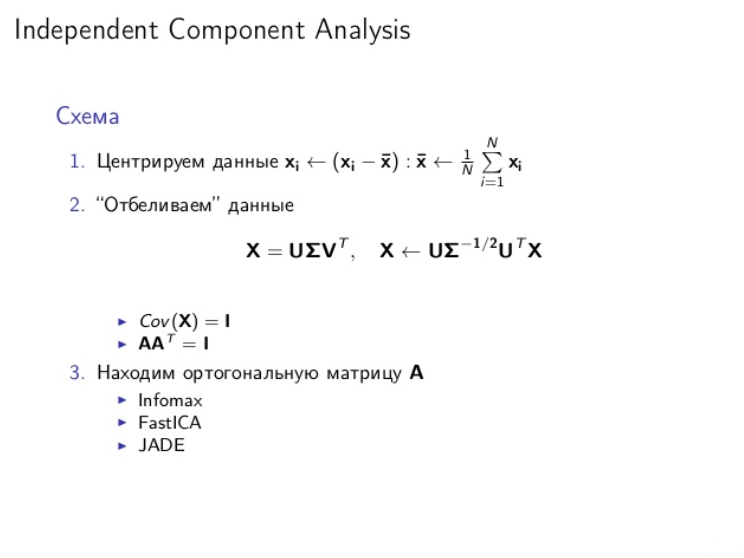
\includegraphics[width=\textwidth]{v14.png}\end{center}\end{frame}
\begin{frame}{ICA -- Анализ независимых компонентов: Схема решения}

\begin{enumerate}
\item Центрируем данные: $x_i \leftarrow (x_i - \bar{x}) : \bar{x} \leftarrow \frac{1}{N} \sum\limits_{i=1}^{N} x_i$\pause
\item Отбеливаем данные

$$X = U \Sigma V, ~ X \leftarrow U \Sigma^{-\frac{1}{2}} U^T X$$

    \begin{itemize}
        \item $Cov(X) = I$
        \item $AA^T = I$
    \end{itemize}

\item Находим ортогональную матрицу $A$

    \begin{itemize}
        \item Infomax
        \item FastICA
        \item JADE
    \end{itemize}
\end{enumerate}

\end{frame}






%\begin{frame}\begin{center}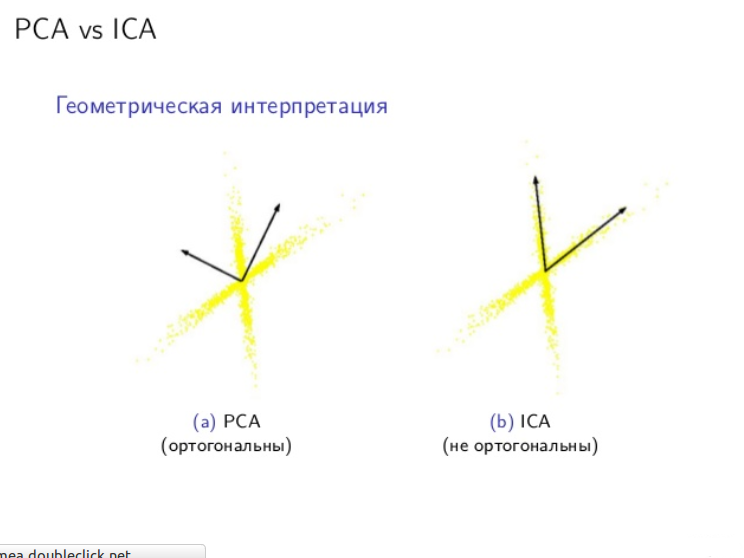
\includegraphics[width=\textwidth]{v15.png}\end{center}\end{frame}

\begin{frame}{PCA vs ICA: Геометрическая интерпретация}
\begin{center}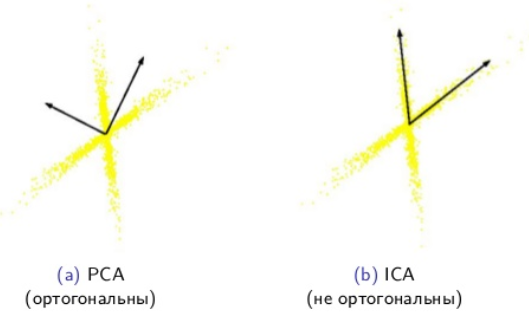
\includegraphics[width=\textwidth]{PCAvsICA.png}\end{center}
\end{frame}

%\begin{frame}\begin{center}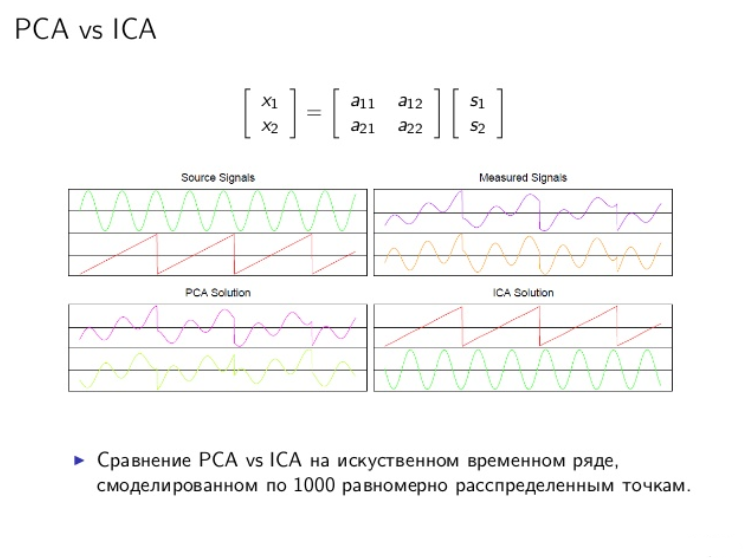
\includegraphics[width=\textwidth]{v16.png}\end{center}\end{frame}
\begin{frame}{PCA vs ICA: Пример}
\begin{center}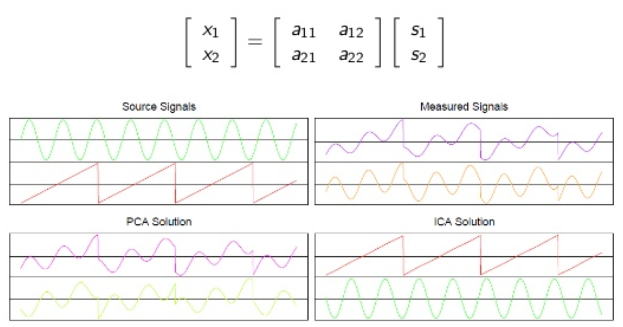
\includegraphics[width=\textwidth]{PCAvsICA_model.png}\end{center}
\end{frame}




\begin{frame}[fragile]{PCA vs ICA: Пример (\href{http://scikit-learn.org/stable/auto_examples/decomposition/plot_ica_blind_source_separation.html}{источник})}

\begin{lstlisting}
np.random.seed(0)
n_samples = 2000
time = np.linspace(0, 8, n_samples)

s1 = np.sin(2 * time)  # Signal 1 : sinusoidal signal
s2 = np.sign(np.sin(3 * time))  # Signal 2 : square signal
s3 = signal.sawtooth(2 * np.pi * time)  # Signal 3: saw tooth signal

S = np.c_[s1, s2, s3]
S += 0.2 * np.random.normal(size=S.shape)  # Add noise

S /= S.std(axis=0)  # Standardize data
# Mix data
A = np.array([[1, 1, 1], [0.5, 2, 1.0], [1.5, 1.0, 2.0]])  # Mixing matrix
X = np.dot(S, A.T)  # Generate observations

# Compute ICA
ica = FastICA(n_components=3)
S_ = ica.fit_transform(X)  # Reconstruct signals
A_ = ica.mixing_  # Get estimated mixing matrix

# We can `prove` that the ICA model applies by reverting the unmixing.
assert np.allclose(X, np.dot(S_, A_.T) + ica.mean_)

# For comparison, compute PCA
pca = PCA(n_components=3)
H = pca.fit_transform(X)  # Reconstruct signals based on orthogonal components
\end{lstlisting}
\end{frame}


\begin{frame}{Результаты слепого разделения сигналов}\begin{center}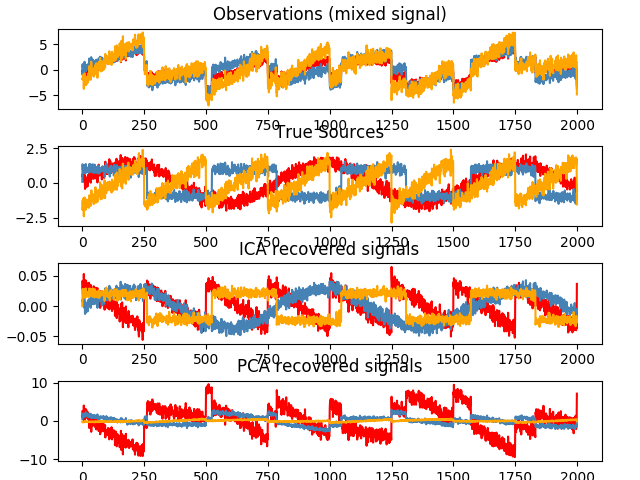
\includegraphics[height=\textheight]{src/1.png}\end{center}\end{frame}
\begin{frame}{Результаты слепого разделения сигналов: Исходные данные}\begin{center}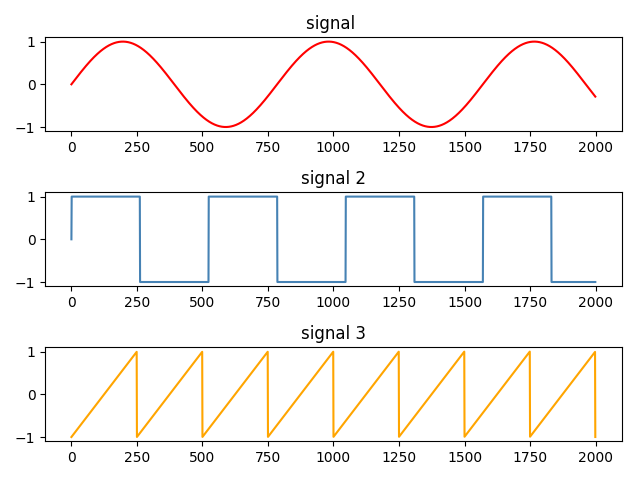
\includegraphics[height=\textheight]{src/2.png}\end{center}\end{frame}
\begin{frame}{Результаты слепого разделения сигналов: Измеренные данные}\begin{center}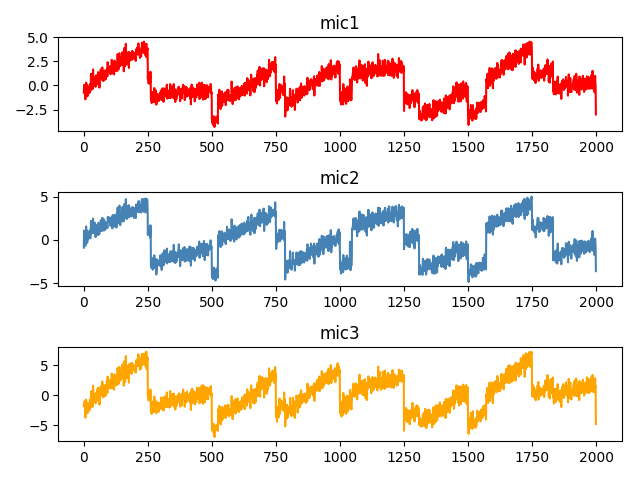
\includegraphics[height=\textheight]{src/3.png}\end{center}\end{frame}
\begin{frame}{Результаты слепого разделения сигналов: ICA}\begin{center}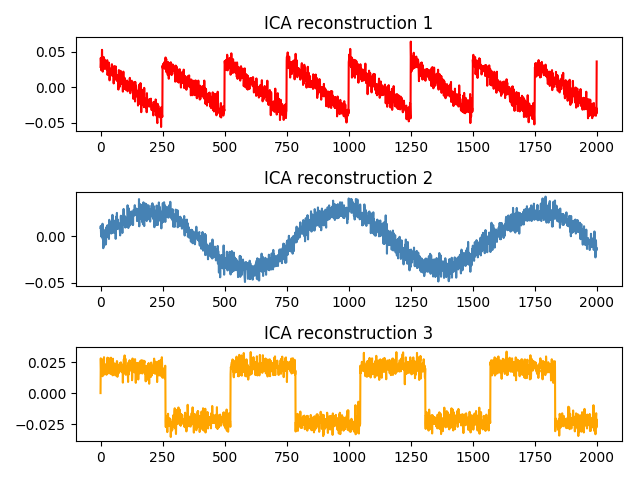
\includegraphics[height=\textheight]{src/3_S_.png}\end{center}\end{frame}
\begin{frame}{Результаты слепого разделения сигналов: PCA}\begin{center}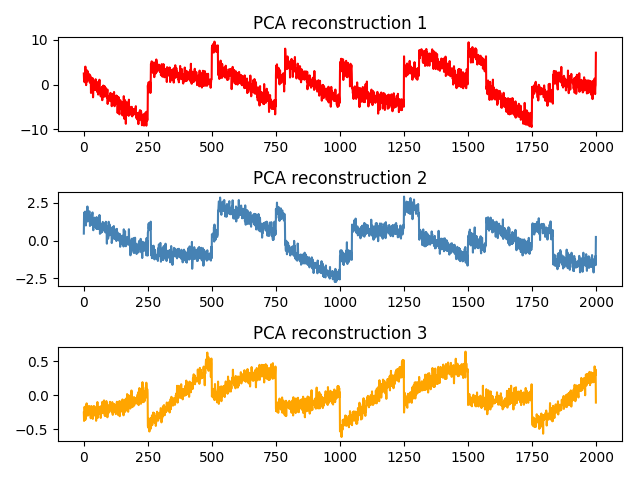
\includegraphics[height=\textheight]{src/3_H.png}\end{center}\end{frame}






\begin{frame}{Применение ICA}\begin{center}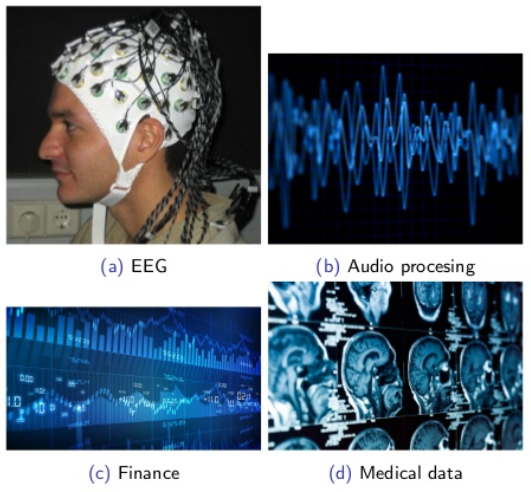
\includegraphics[height=\textheight]{ICA_Use.png}\end{center}\end{frame}





\subsection{Autoencoders}

\begin{frame}\begin{center}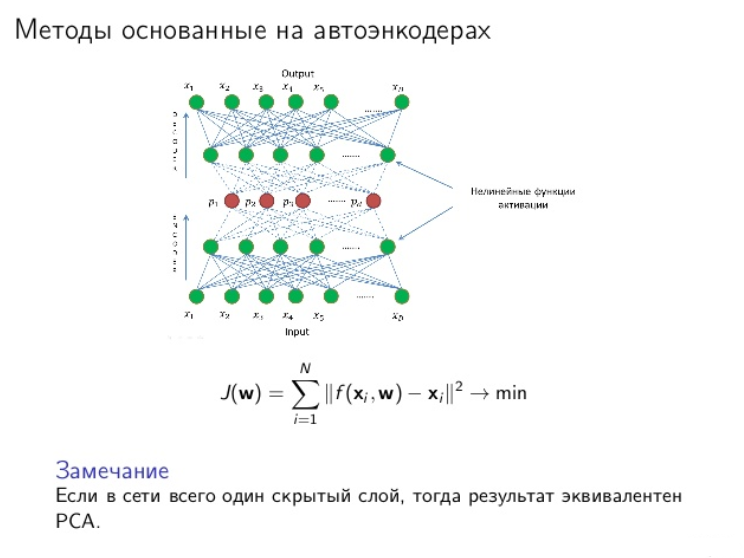
\includegraphics[width=\textwidth]{v18.png}\end{center}\end{frame}
\begin{frame}\begin{center}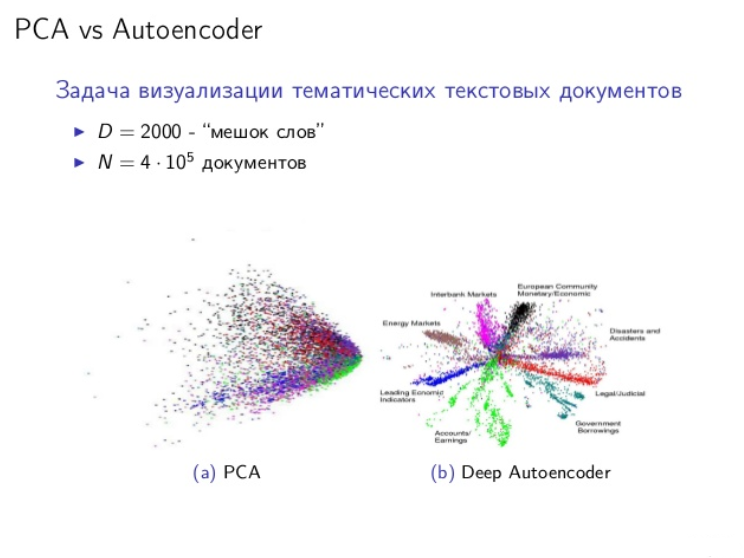
\includegraphics[width=\textwidth]{v19.png}\end{center}\end{frame}
\begin{frame}\begin{center}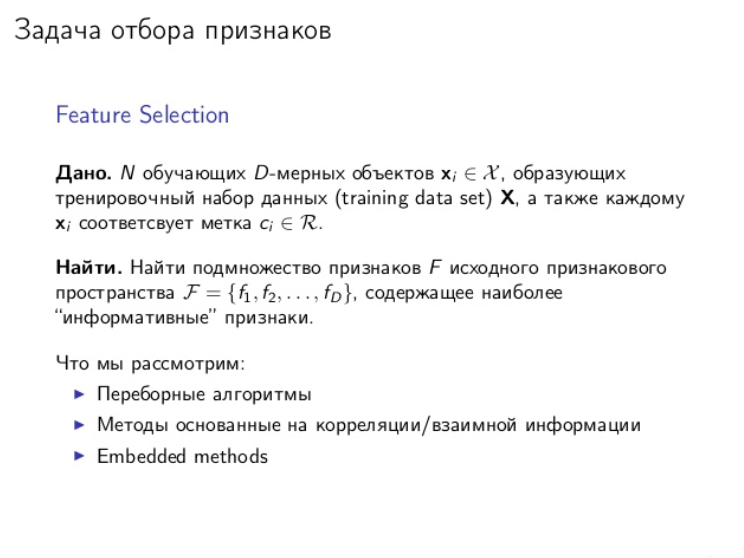
\includegraphics[width=\textwidth]{v21.png}\end{center}\end{frame}
\begin{frame}\begin{center}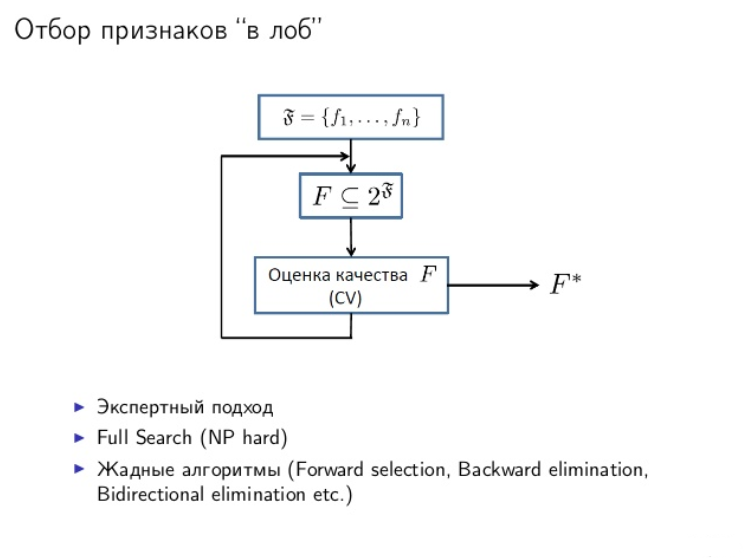
\includegraphics[width=\textwidth]{v22.png}\end{center}\end{frame}
\begin{frame}\begin{center}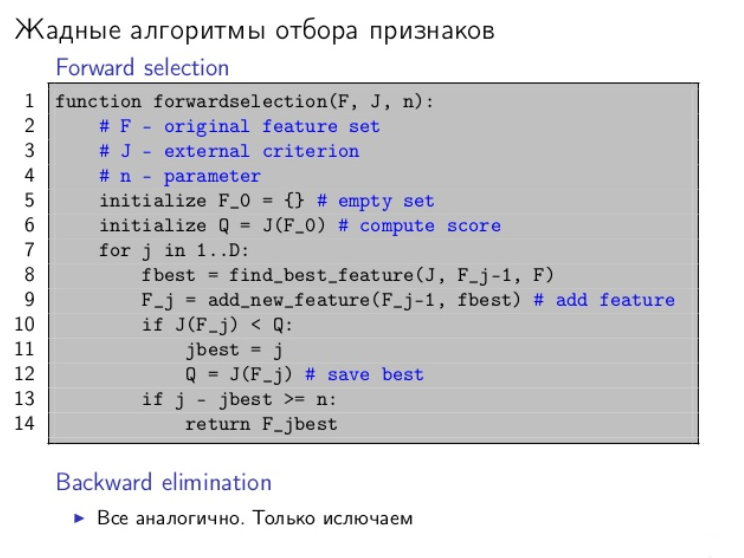
\includegraphics[width=\textwidth]{v23.png}\end{center}\end{frame}
\begin{frame}\begin{center}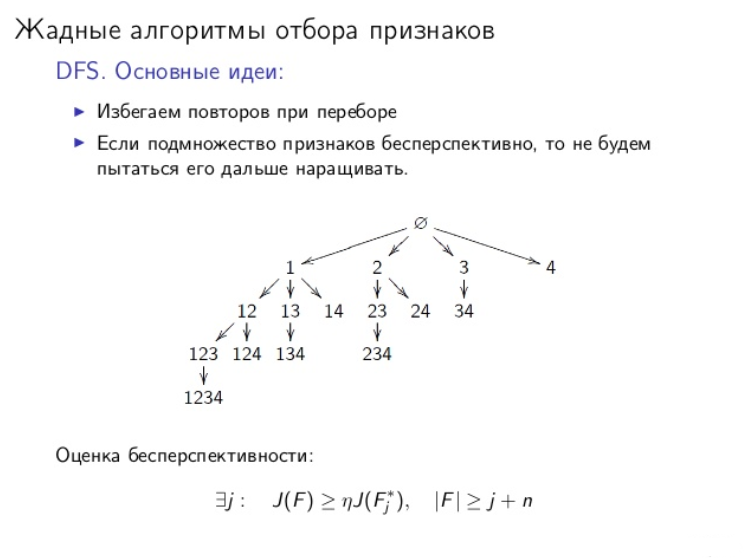
\includegraphics[width=\textwidth]{v24.png}\end{center}\end{frame}

%\begin{frame}\begin{center}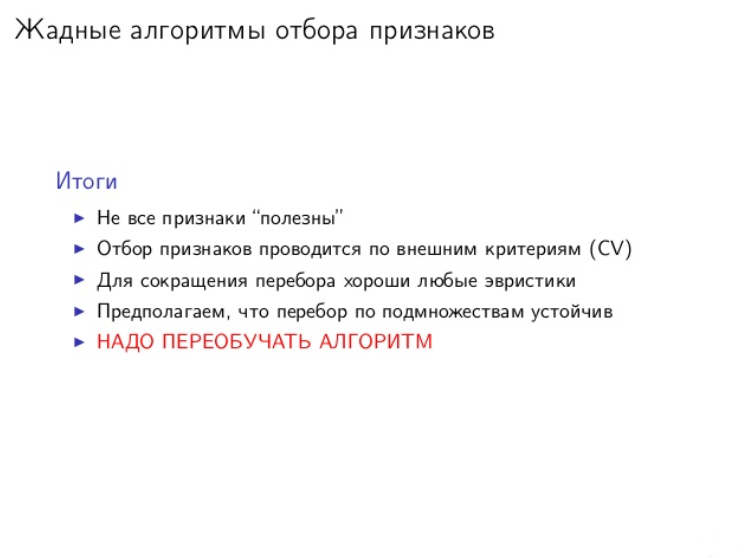
\includegraphics[width=\textwidth]{v25.png}\end{center}\end{frame}
%\begin{frame}\begin{center}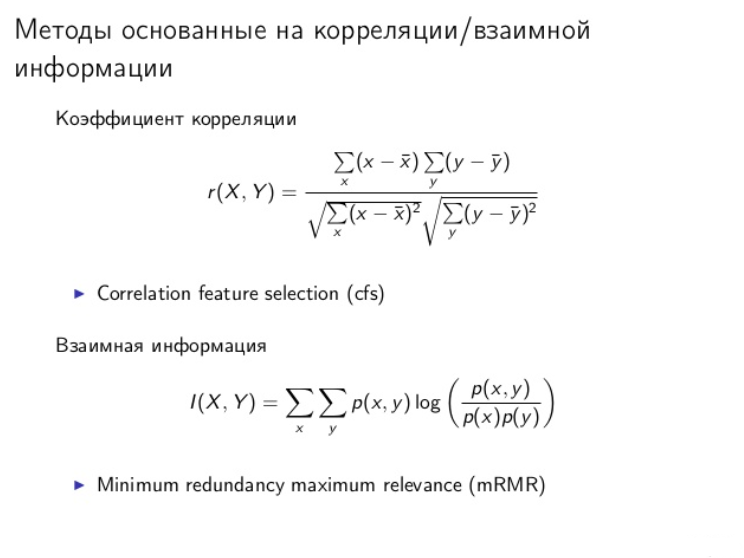
\includegraphics[width=\textwidth]{v26.png}\end{center}\end{frame}
%\begin{frame}\begin{center}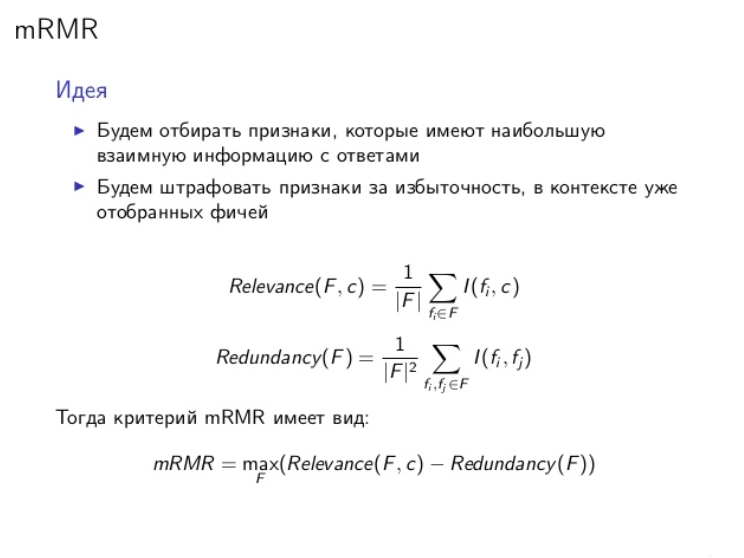
\includegraphics[width=\textwidth]{v27.png}\end{center}\end{frame}
%\begin{frame}\begin{center}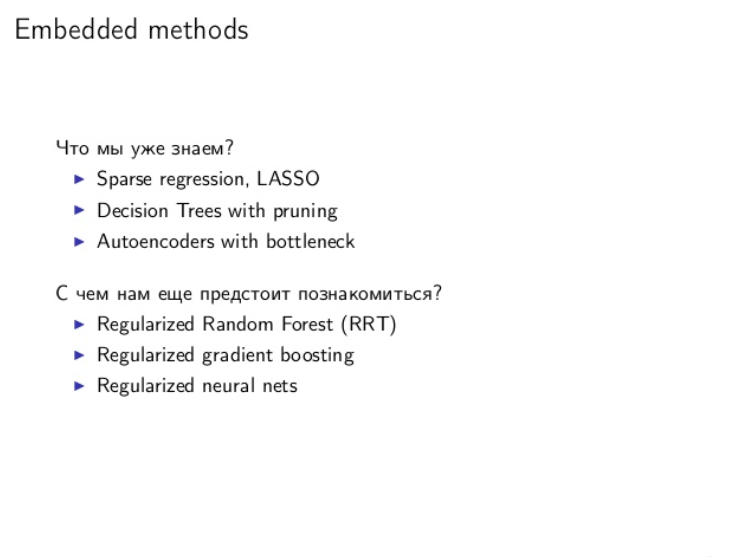
\includegraphics[width=\textwidth]{v28.png}\end{center}\end{frame}


\begin{frame}{Выводы по <<жадным>> алгоритмам формирования признаков}
\begin{itemize}
\item не всё то -- признак, что -- блестит (не все признаки полезны)\pause
\item отбор признаков происходит по внешним критериям\pause
\item любые эвристики хороши для сокращения перебора\pause
\item ...при условии что перебор устойчив по подмножествам признаков\pause
\item если не делать никакой декомпозиции, {\color{red}постоянно нужно переобучать алгоритм под новые данные}
\end{itemize}
\end{frame}



\stepcounter{section}
\repeatSectionTitle[Спасибо за внимание!]

\end{document}
